\section{Results}

\subsection{Search Outcomes}
Table~\ref{tab:configs} reports the validation loss for every searched configuration at a matched horizon.
Three architectural perturbations---increased depth (S2-02), more KV heads (S2-03), and tied embeddings (S2-04)---offer no short-horizon gain and are discarded, leaving the baseline architecture unchanged.
Among learning-rate candidates, $3\times10^{-4}$ (S3-01) beats both the baseline $6\times10^{-4}$ and $1\times10^{-3}$, while widening the WSD ratio to $20\%$ (S3-02) yields no further improvement.
Consequently, the winning configuration differs from the baseline by a \emph{single} change: a lower stable-phase learning rate.

\begin{table}[htbp]
\centering
\caption{Search outcomes. Loss is reported at a matched horizon (\textbf{80} steps for S2/S3; \textbf{160} steps for S4).}
\label{tab:configs}
\begin{tabular}{llccc}
\toprule
\textbf{ID} & \textbf{Change vs.\ best} & \textbf{LR} & \textbf{Val.\ loss} & \textbf{Outcome} \\
\midrule
S1-01 & baseline & $6$e$-$4 & 5.962@80 & baseline \\
S2-01 & LR $1$e$-$3 & $1$e$-$3 & 6.019@80 & worse \\
S2-02 & layers $24\to28$ & $6$e$-$4 & 6.119@80 & worse \\
S2-03 & KV heads $2\to4$ & $6$e$-$4 & 5.979@80 & no gain \\
S2-04 & embeddings tied & $6$e$-$4 & 6.030@80 & worse \\
S3-01 & LR $3$e$-$4 & $3$e$-$4 & 5.908@80 & \textbf{best} \\
S3-02 & WSD $10\%\to20\%$ & $3$e$-$4 & 5.917@80 & no gain \\
\midrule
S4-01 & winner, 160 steps & $3$e$-$4 & \textbf{4.969}@160 & \textbf{winner} \\
 & baseline, 160 steps & $6$e$-$4 & 5.086@160 & reference \\
\bottomrule
\end{tabular}
\end{table}

\subsection{Winning Configuration}
The verification run (S4-01) retrains the S3 winner from scratch for $160$ steps and reaches a validation loss of \textbf{4.969}, versus $5.086$ for the baseline at the same step count---an improvement of $-0.117$ attributable solely to lowering the stable learning rate from $6\times10^{-4}$ to $3\times10^{-4}$.
The $80$-step reproduction ($5.8995$) matches the S3-01 result ($5.908$) within run-to-run noise, confirming the recipe is reproducible from scratch.

\subsection{Training Dynamics}
Figure~\ref{fig:loss} shows the baseline (S1-01) training-loss curve over $300$ steps.
Loss decreases smoothly from $\approx$12.1 to $3.59$; the final bend corresponds to the exponential WSD decay phase, during which the learning rate anneals to its minimum.
This confirms that the WSD schedule converges cleanly under the selected hyper-parameters without instability.

\begin{figure}[htbp]
\centering
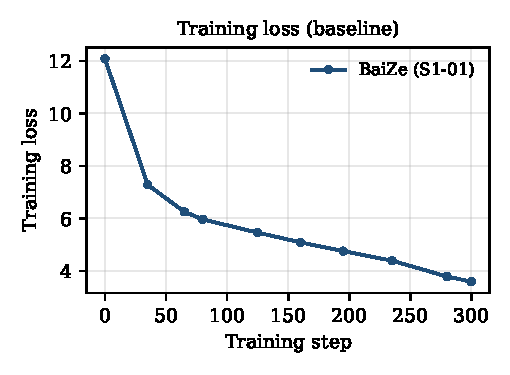
\includegraphics[width=\columnwidth]{figures/train_loss.pdf}
\caption{Training loss of the baseline (S1-01) over 300 steps. The final bend marks the exponential WSD decay phase.}
\label{fig:loss}
\end{figure}

Figure~\ref{fig:ablation} summarises the short-horizon (80-step) losses across swept configurations, visualising the two clear findings: the architecture is already optimal, and the only productive lever is the stable learning rate.

\begin{figure}[htbp]
\centering
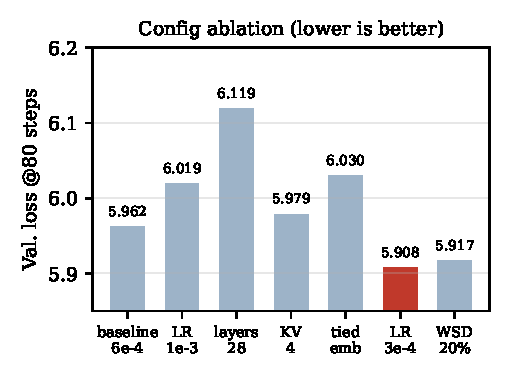
\includegraphics[width=\columnwidth]{figures/config_ablation.pdf}
\caption{Short-horizon (80-step) validation loss across swept configurations. Lower is better. The winning configuration (S3-01) is highlighted.}
\label{fig:ablation}
\end{figure}

\subsection{Architecture Selection Evidence at 2B}\label{sec:arch2b}
To anchor the architecture choice (Section~\ref{sec:arch-rationale}) in controlled experiment rather than availability alone, we trained two candidate 2B backbones---MiniCPM5-2B (dense) and Mamba2-hybrid (Nemotron-H style)~\cite{dao2024transformers,nvidia2025nemotronh}---from scratch under identical data, seed, and 6-GPU (TP1/DP6) settings for 1000 steps, then profiled inference with a shared mcore direct driver.
Table~\ref{tab:arch2b} reports the three-way comparison: the hybrid wins two of three axes---lower loss with fewer parameters, and faster inference---while the dense model retains a $\sim$24\% training-throughput edge.
This positions Mamba2-hybrid as the preferred 2B backbone for inference-heavy deployments, while the dense GQA design stays optimal for the budget-constrained 1B agent built here.
The dense model's low decode rate is a mcore direct-driver artefact (per-layer fused-attention CPU launch overhead, CPU-bound) rather than a fundamental inefficiency; both backbones share the same measurement path, so the relative decode comparison ($\times$10.3) remains trustworthy.

\begin{table}[htbp]
\centering
\caption{Matched 2B-scale dense-vs-hybrid comparison (1000 steps, seq 4096, GBS 6, TP1/DP6, BF16; inference: mcore direct driver, TP1, BF16, seq-2048 prompt + 256 gen).}
\label{tab:arch2b}
\begin{tabular}{lccc}
\toprule
\textbf{Metric} & \textbf{MiniCPM5-2B} & \textbf{Mamba2-hybrid} & \textbf{Winner} \\
\midrule
Parameters & 2.512B & \textbf{2.220B} & hybrid ($-11.6\%$) \\
Final loss (1000 steps) & 4.8065 & \textbf{4.6846} & hybrid \\
Training tok/s (6 cards) & \textbf{$\sim$89k} & $\sim$72k & dense ($+24\%$) \\
Prefill tok/s & 21{,}436 & \textbf{23{,}692} & hybrid ($+10.5\%$) \\
Decode tok/s & 2.21 & \textbf{22.77} & hybrid ($\times$10.3) \\
\bottomrule
\end{tabular}
\end{table}